\chapter{火球、参考系与四维矢量}

我们从高能碰撞讨论中遗留的一个问题开始。两个重核的碰撞产生的是一个剧烈变化的对象，而不是一个宁静的天文黑洞。那么，用视界来描述这种碰撞究竟意味着什么？答案将经由强耦合物质的五维图像、一组关于加速器的实际问题，最终回到狭义相对论的几何。到结束时，速度和动量已成为四维矢量，而能量则在动量的三个分量旁边占据了自己的位置。

\section{第五维中的火球}

\begin{classroomqa}
\audiencequestion{碰撞中产生的对象是不稳定的，并且会改变形状。这样一个复杂的对象怎么能被称为黑洞呢？}
\lecturerresponse{设想第五个空间方向在地板与天花板之间延伸。该方向上的引力将激发态拉向地板。碰撞在那里沉积了一团炽热的能量块；这团能量块会扩散并改变形状，但它仍然可以拥有视界、温度和熵。}
\end{classroomqa}

设想粒子，或者更形象地说，小弦，在这个五维世界中运动。落到地板上的激发态在四维中表现为强子：质子、中子、介子以及其他延展的复合对象。附着在天花板附近的激发态则显得更为基本。因此，竖直位置是一种几何化地编码标度的方式：地板代表长距离的强子区域，而天花板代表短距离的自由度。

当两个强子碰撞时，地板附近的两个对象相互撞击，溅射出大量能量。结果并不是一个刚体。它是一个炽热的、带有视界的能量块，是五维引力场中的一种水洼。它既不是普通四维空间中的天文黑洞，也不是附着在天花板上的普朗克尺度黑洞。它是地板附近强相互作用火球的引力描述。

在高能下，入射核被洛伦兹收缩成薄饼状。它们碰撞，将能量沉积在一个小区域中，并产生一种向平衡态扩散的流体。其微小的黏滞性是夸克--胶子等离子体令人惊讶的特征之一。在五维描述中，同样的演化就是扭曲视界的弛豫。

\begin{figure}[H]
\centering
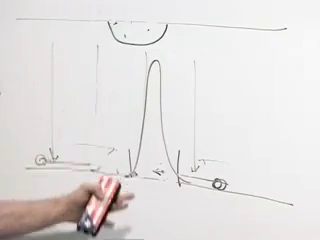
\includegraphics[width=0.82\textwidth]{lecture_05_figure_01.png}
\caption{第五维的地板与天花板图像。碰撞后，中央带有视界的能量块沿地板扩散。}
\lectureframe{00:04:22}
\end{figure}

视界不会永远存在。霍金辐射会带走能量，而在四维描述中，这种辐射就是从碰撞中涌现出的普通强子簇射。用这种语言来说，探测器事件中的数千条径迹就是从对偶黑洞中蒸发出的粒子。

\subsection{额外维度是真实的吗？}

\begin{classroomqa}
\audiencequestion{第五维是一个空间维度吗？地板与天花板之间画出的那条线是否真的沿该方向延伸？}
\lecturerresponse{是的。它是类空的，而在那个五维几何中画出的曲面就是一个视界。至于人们是把额外方向称为``真实的''，还是把它视为一种等价的数学描述，则是一个更深层的问题。}
\end{classroomqa}

有用的陈述并不是引力取代了量子色动力学。相反，两种语言可以描述同一物理。在四维语言中，存在一个由夸克和胶子组成的炽热火球，没有普通的引力场。在五维语言中，则存在引力和一个视界。如果这种对应关系是正确的，那么诚实的QCD计算和对偶引力计算在两者都能进行的地方必须一致。

\begin{classroomqa}
\audiencequestion{QCD既没有引力也没有视界。黑洞图像是在添加新物理，还是仅仅重新描述了火球？}
\lecturerresponse{在四维中，它是夸克和胶子的等离子体；在五维化身中，它有一个带视界的引力描述。优势在于计算。强耦合QCD极其困难，而某些视界性质---尤其是黏滞性---则相对容易计算。}
\end{classroomqa}

``真实维度''与``数学类比''之间的区分不必在描述变得有用之前就得到解决。当一个结构与其他变量结合成一组更简单、更连贯的定律时，它就获得了物理解释。尽管如此，人们不应夸大这一点：规范/引力对偶性对所观测到的夸克--胶子等离子体的应用，是强耦合动力学的模型，而不是证明现实世界中的QCD具有已知的精确引力对偶。\editorialnote{这一限定明确了QCD应用的现代地位；它并不改变此处所发展的五维机制。}

\section{为什么对撞机使束流对撞}

现在这些问题变得实际了。为什么要使用两束运动的束流，而不是一束束流加一个静止靶？为什么环形加速器如此之大？为什么电子和质子的处理方式不同？所有这些问题都是关于相对论能量的问题。

\begin{classroomqa}
\audiencequestion{为什么要让两束束流对撞，而不是将一束高能束流射向静止靶？}
\lecturerresponse{产生新粒子的是质心系中可用的能量。两束相等且方向相反的相对论束流没有净动量，因此它们的能量基本上全部可用于碰撞。固定靶则迫使大部分入射能量保留为质心的运动。}
\end{classroomqa}

对于两个具有大小为\(p\)的相反动量的超相对论粒子，在\(c=1\)单位下的讲义级估计为
\begin{equation}
E_{\mathrm{cm}}^{\mathrm{collider}}\simeq 2p.
\end{equation}
相应的固定靶估计仅按束流动量的平方根增长，
\begin{equation}
E_{\mathrm{cm}}^{\mathrm{fixed}}\sim \sqrt{mp}.
\end{equation}
关键在于这种标度关系，而不是被省略的数值因子：将束流能量加倍会使对撞机能量加倍，但只会使固定靶质心能量增加一个平方根。

不变量计算使比较变得精确。如果\(P_1\)和\(P_2\)是入射四维动量，那么
\begin{equation}
s=(P_1+P_2)^2,
\qquad E_{\mathrm{cm}}=\sqrt{s}.
\end{equation}
对于能量为\(E\)的等量反向传播束流，空间动量相互抵消，且\(\sqrt{s}=2E\)。对于能量为\(E\gg m\)的抛射粒子撞击静止的等质量靶，
\begin{equation}
s=2m^2+2mE,
\qquad
\sqrt{s}\simeq \sqrt{2mE}
\qquad (c=1).
\end{equation}
这一简短的不变量推导提供了口头估计中被压低的因子。\editorialnote{引入该推导是为了使讲义的标度论证可复现。}

\begin{classroomqa}
\audiencequestion{环形加速器必须如此之大，是否有根本原因？同一束流能否只是更多次地通过一台更小的机器循环？}
\lecturerresponse{场和材料施加了限制。粒子每米获得的能量增量是有限的，因此更高能量的机器需要更长的有效加速长度。紧凑的圆环还要求更大的横向加速度，而加速电荷会辐射。如果环太小，束流辐射能量的速度就会与机器供给能量的速度一样快。}
\end{classroomqa}

偏转关系近似为
\begin{equation}
p=qBR,
\end{equation}
因此对于固定的磁场\(B\)，更大的动量\(p\)需要更大的半径\(R\)。射频腔完成提高束流能量的功；磁铁使束流偏转并聚焦。广泛的教训仍然是黑板上给出的那一条：场强和辐射损失阻止我们将任意高能的加速器压缩成一个小环。

圆周运动即使在速率恒定时也有加速度，因为速度方向在改变。加速电荷会发射同步辐射。直线加速器避免了连续的偏转损失，尽管短的加速推动本身并非字面意义上的无辐射。环形机器接受偏转代价，以换取在每一圈上重复使用同一套装置。

\begin{classroomqa}
\audiencequestion{为什么电子与SLAC的直线机器相关联，而环形高能对撞机使用质子或其他强子？}
\lecturerresponse{电子要轻得多。在给定的高能量下，它们的洛伦兹因子大得多，而圆周加速使它们辐射得强烈得多。较重的质子可以反复循环，在每一圈上获得能量，直到同步辐射损失变得不可承受。}
\end{classroomqa}

对于固定的能量和环半径，辐射功率随粒子质量极其陡峭地变化，
\begin{equation}
P_{\mathrm{sync}}\propto \frac{E^4}{m^4R^2}.
\end{equation}
这就是为什么电子--质子之别远比``较轻的粒子运动得更快''这一说法所暗示的要鲜明得多：两束束流都可以已经极其接近\(c\)，但它们的洛伦兹因子和辐射损失却非常不同。\editorialnote{弯曲关系和同步辐射标度律使讲座中定性的加速器论证变得精确；这些并未在黑板上推导出来。}

\begin{classroomqa}
\audiencequestion{为什么不也把强子放在直线中加速呢？}
\lecturerresponse{可以。困难在于长度。在环中，同一粒子会多次经过加速结构；一台等效的直线强子机器则必须极其长。有用的折中方案是一个大环，大到质子辐射仍然可以容忍。}
\end{classroomqa}

这些加速器问题恰恰暴露出牛顿规则为何不够用。我们现在回到狭义相对论，并建立使这类比较系统化的语言。

\section{车库与加长轿车}

考虑一个约十二英尺长的车库和一辆约二十英尺长的加长轿车。司机不断加速，直到加长轿车发生洛伦兹收缩，希望它能装得下。在车库参考系中，运动中的加长轿车更短，所以看起来是可能的。然而在加长轿车参考系中，运动中的车库更短，所以看起来是不可能的。整辆加长轿车能同时位于车库内吗？

把两扇门都打开，这样就不会因撞到墙而分散我们的注意力。说加长轿车在里面，意味着它的前端和后端\emph{同时}都在里面。最后这个词包含了整个谜题。

画一个时空图，\(t\)竖直，\(x\)水平。在\(c=1\)单位下，光线构成\(45^\circ\)光锥。车库静止，所以它两扇门的世界线是竖直的。加长轿车的前端和后端描出两条平行的倾斜世界线。运动参考系的\(t'\)轴朝光锥方向倾斜，其同时性直线平行于倾斜的\(x'\)轴。

\begin{figure}[H]
\centering
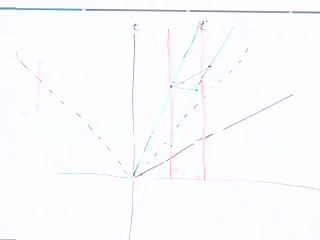
\includegraphics[width=0.82\textwidth]{lecture_05_figure_02.png}
\caption{完整的车库--加长轿车时空图。竖直线界定车库；斜线描出加长轿车的两端。水平切片和倾斜切片表示两个参考系不同的同时性切片。}
\lectureframe{00:31:05}
\end{figure}

在车库参考系中，一条水平线可以在两条车库世界线之间穿过两条加长轿车世界线。在那个车库时刻，后端已经进入，而前端尚未离开。收缩后的加长轿车完全在里面。

在加长轿车参考系中，相关的同时事件位于一条倾斜线上。过后端进入这一事件画这样一条线。它与前端世界线相交时，前端已经越过了远端那扇门。按照它自己的同时性，加长轿车从未完全在里面。两种说法都成立，因为它们比较的是不同的两对事件。

\begin{classroomqa}
\audiencequestion{两条绿色世界线以及它们之间的水平线段是否构成一个平行四边形？那条黑色线段是车辆的长度吗？}
\lecturerresponse{水平线段是洛伦兹收缩后的长度，因为它的端点在车库参考系中同时。固有长度则由在加长轿车参考系中同时的端点得到，位于平行于\(x'\)的直线上。这两种测量使用穿过同一对世界线的不同切片。}
\end{classroomqa}

如果\(L_0\)是固有长度，那么车库参考系中的水平切片长度为\begin{equation}
L=\frac{L_0}{\gamma},
\qquad
\gamma=\frac{1}{\sqrt{1-v^2/c^2}}.
\end{equation}
仅凭公式并不能解决这个悖论。图可以，因为它显示了比较的是哪些事件。每当一个相对论谜题似乎产生两个不相容的答案时，都要寻找对``同时''的未明言使用。

\section{四个坐标与两个指标位置}

要从谜题走向运动定律，我们需要一种能记住几何的记号。把坐标打包为
\begin{equation}
(X^1,X^2,X^3,X^0)=(x,y,z,t),
\qquad X^\mu=(x,y,z,t),
\end{equation}
其中\(\mu\)取遍\(1,2,3,0\)。这种排序把时间放在页面最后，尽管它的指标是\(0\)，与黑板上使用的约定一致。

\begin{classroomqa}
\audiencequestion{我们是在设定\(c=1\)吗？如果恢复普通单位，时间坐标是否应为\(ct\)？}
\lecturerresponse{是的。我们在展开几何时设定\(c=1\)，并在量纲或非相对论极限重要时把\(c\)的因子放回去。采用常规长度单位时，时间坐标是\(ct\)。}
\end{classroomqa}

同一个矢量也可以用下指标写出。按照这里采用的符号约定，
\begin{equation}
X_\mu=(-x,-y,-z,t).
\end{equation}
因此，降低一个指标会反转三个空间分量的符号，而时间分量保持不变。例如，
\begin{equation}
X^\mu=(3,2,4,10)
\quad\Longrightarrow\quad
X_\mu=(-3,-2,-4,10).
\end{equation}
这并不是两个时空点；它们是同一个几何对象的两种分量形式。

\begin{classroomqa}
\audiencequestion{哪些分量是协变的，哪些是逆变的，这些标记应该是上标还是下标？}
\lecturerresponse{上指标分量是逆变的；下指标分量是协变的。来自课堂的一个有用记忆法是``co 是低，contra 是高。''物理学家常常直接说“楼上”和“楼下”。}
\end{classroomqa}

这种记号在不变缩并中体现了其价值
\begin{equation}
X_\mu X^\mu=t^2-x^2-y^2-z^2.
\label{eq:l5-interval}
\end{equation}
用微分形式表示，这就是
\begin{equation}
d\tau^2=dt^2-dx^2-dy^2-dz^2
\qquad (c=1).
\label{eq:l5-proper-time}
\end{equation}
对于类时运动，\(d\tau\) 是沿世界线运动的时钟所记录的时间。

只要同一个指标在上方出现一次、在下方出现一次，就理解为对它求和。爱因斯坦约定把
\begin{equation}
\sum_{\mu}X_\mu X^\mu
\end{equation}
变成式~\eqref{eq:l5-interval}中更短的表达式。这不仅仅是排版上的节省。它防止闵可夫斯基几何中交替出现的符号在每一个方程中都被手工重写。

\begin{classroomqa}
\audiencequestion{\(\tau\) 是固有时（proper time）的标准符号吗？}
\lecturerresponse{是的。符号 \(s\) 有时也会被使用，但 \(\tau\) 是固有时的标准选择。}
\end{classroomqa}

\section{作为简单对称性的旋转}

洛伦兹助推混合空间和时间。在研究那个矩阵之前，先考虑更熟悉的操作：旋转空间坐标轴。如果相对运动指向任意方向，我们可以旋转坐标轴，直到该方向成为新的 \(x\) 轴，然后施加已知的助推。因此，旋转是这一构造的一部分，而不是装饰性的绕路。

对于绕 \(z\) 轴旋转角度 \(\theta\)，
\begin{align}
x'&=x\cos\theta+y\sin\theta,\nonumber\\
y'&=-x\sin\theta+y\cos\theta,\label{eq:l5-rotation}\\
z'&=z.\nonumber
\end{align}
在 \(\theta=0\) 时，这些方程给出 \(x'=x\) 和 \(y'=y\)；在 \(\theta=\pi/2\) 时，它们以预期的符号交换坐标轴。

该变换保持欧几里得距离不变。记
\(c_\theta=\cos\theta\) 和 \(s_\theta=\sin\theta\)，
\begin{align}
x'^2+y'^2
&=(xc_\theta+ys_\theta)^2+(-xs_\theta+yc_\theta)^2\nonumber\\
&=x^2(c_\theta^2+s_\theta^2)
  +y^2(s_\theta^2+c_\theta^2)\nonumber\\
&\quad+2xyc_\theta s_\theta-2xyc_\theta s_\theta\nonumber\\
&=x^2+y^2.
\end{align}
交叉项相消，且 \(c_\theta^2+s_\theta^2=1\)。由于 \(z'=z\)，整个长度 \(x^2+y^2+z^2\) 不变。

同样的方程可以写成一个矩阵方程：
\begin{equation}
\begin{pmatrix}x'\\y'\\z'\end{pmatrix}
=
\underbrace{\begin{pmatrix}
\cos\theta&\sin\theta&0\\
-\sin\theta&\cos\theta&0\\
0&0&1
\end{pmatrix}}_{M}
\begin{pmatrix}x\\y\\z\end{pmatrix}.
\label{eq:l5-rotation-matrix}
\end{equation}
用指标记号表示，
\begin{equation}
x'^i=M^i{}_{j}x^j,
\qquad i,j=1,2,3.
\end{equation}

\begin{figure}[H]
\centering
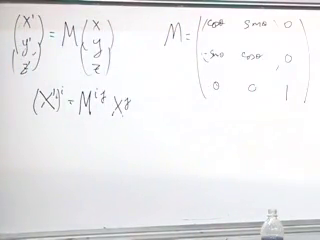
\includegraphics[width=0.82\textwidth]{lecture_05_figure_03.png}
\caption{空间旋转既写成矩阵方程，也写成指标记号。}
\lectureframe{01:00:40}
\end{figure}

\section{洛伦兹矩阵与速度合成}

对于沿 \(x\) 方向的运动，在 \(c=1\) 单位下的洛伦兹变换为
\begin{align}
x'&=\gamma_v(x-vt), & y'&=y,\nonumber\\
z'&=z, & t'&=\gamma_v(t-vx),
\end{align}
其中
\begin{equation}
\gamma_v=\frac{1}{\sqrt{1-v^2}}.
\end{equation}
采用分量顺序 \((x,y,z,t)\)，这变为
\begin{equation}
\begin{pmatrix}x'\\y'\\z'\\t'\end{pmatrix}
=
\begin{pmatrix}
\gamma_v&0&0&-\gamma_vv\\
0&1&0&0\\
0&0&1&0\\
-\gamma_vv&0&0&\gamma_v
\end{pmatrix}
\begin{pmatrix}x\\y\\z\\t\end{pmatrix}.
\label{eq:l5-lorentz-matrix}
\end{equation}

\begin{figure}[H]
\centering
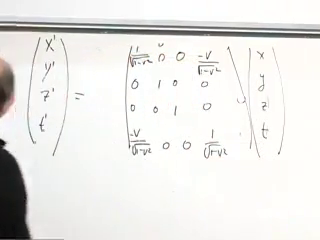
\includegraphics[width=0.82\textwidth]{lecture_05_figure_04.png}
\caption{\(4\times4\) 洛伦兹矩阵。只有 \(x\) 和 \(t\) 分量混合；\(y\) 和 \(z\) 保持不变。}
\lectureframe{01:04:40}
\end{figure}

矩阵乘法现在回答一个物理问题。假设一个观察者相对于我们以速度 \(v\) 运动，而第三个观察者相对于该观察者以速度 \(u\) 运动，全都沿同一轴。牛顿运动学会给出 \(w=u+v\)，这会使两个 \(3c/4\) 的速度合成为 \(3c/2\)。相对论必须给出不同的规则。

助推的有效部分是 \(2\times2\) 矩阵
\begin{equation}
B(v)=\gamma_v
\begin{pmatrix}1&-v\\-v&1\end{pmatrix}.
\end{equation}
将两个助推复合得到
\begin{align}
B(u)B(v)
&=\gamma_u\gamma_v
\begin{pmatrix}1&-u\\-u&1\end{pmatrix}
\begin{pmatrix}1&-v\\-v&1\end{pmatrix}\nonumber\\
&=\gamma_u\gamma_v
\begin{pmatrix}
1+uv&-(u+v)\\
-(u+v)&1+uv
\end{pmatrix}.
\label{eq:l5-composed-boost}
\end{align}
非对角元与对角元之比确定了合成助推的速度：
\begin{equation}
w=\frac{u+v}{1+uv}
\qquad(c=1).
\end{equation}
恢复量纲后，
\begin{equation}
w=\frac{u+v}{1+uv/c^2}.
\label{eq:l5-velocity-addition}
\end{equation}

\begin{figure}[H]
\centering
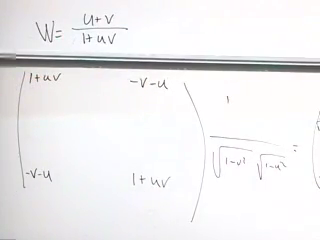
\includegraphics[width=0.82\textwidth]{lecture_05_figure_05.png}
\caption{复合助推矩阵以及自然单位下的速度 \(w=(u+v)/(1+uv)\)。}
\lectureframe{01:15:35}
\end{figure}

如果 \(u\) 和 \(v\) 都接近 \(c\)，则分子趋近 \(2c\)，而分母趋近 \(2\)，所以 \(w\) 趋近 \(c\)，而不是 \(2c\)。更一般地，式~\eqref{eq:l5-velocity-addition}把亚光速输入映射为亚光速结果。矩阵乘法自动编码了速度极限。

\section{四维矢量与普通速度的失效}

四维矢量是任何其四个分量在旋转和洛伦兹助推下与时空坐标以相同方式变换的对象。如果 \(V^\mu\) 是四维矢量，那么按照我们的符号约定
\begin{equation}
V_\mu=(-V^1,-V^2,-V^3,V^0),
\end{equation}
其不变模长为
\begin{equation}
V_\mu V^\mu=(V^0)^2-(V^1)^2-(V^2)^2-(V^3)^2.
\end{equation}
对于两个四维矢量 \(V^\mu\) 和 \(W^\mu\)，缩并
\begin{equation}
W_\mu V^\mu
=W^0V^0-W^1V^1-W^2V^2-W^3V^3
\end{equation}
同样不变。分量在不同参考系之间改变；缩并则不变。

普通速度只有三个分量，
\begin{equation}
\mathbf v=\left(\frac{dx}{dt},\frac{dy}{dt},\frac{dz}{dt}\right).
\end{equation}
附加 \(dt/dt=1\) 并不能使它成为有用的四维矢量。第四个分量
将是平凡的，而且所得对象在洛伦兹变换下不会线性变换。坐标时 \(t\) 从一个参考系到
另一个参考系会改变，因此对 \(t\) 求导会破坏所期望的变换律。

固有时提供了解决办法。沿一条世界线定义
\begin{equation}
u^\mu=\frac{dX^\mu}{d\tau}.
\label{eq:l5-four-velocity}
\end{equation}
微分 \(dX^\mu\) 是四维矢量，而 \(d\tau\) 是不变量，所以
二者之比是四维矢量。形容词 ``固有'' 指的是
分母中的时钟。

链式法则将这个对象与普通速度联系起来：
\begin{equation}
\frac{dx}{d\tau}=\frac{dx}{dt}\frac{dt}{d\tau},
\end{equation}
对 \(y\) 和 \(z\) 也类似。由
式~\eqref{eq:l5-proper-time}，
\begin{align}
\left(\frac{d\tau}{dt}\right)^2
&=1-\left(\frac{dx}{dt}\right)^2
    -\left(\frac{dy}{dt}\right)^2
    -\left(\frac{dz}{dt}\right)^2\nonumber\\
&=1-v^2
\qquad(c=1),
\end{align}
因此
\begin{equation}
\frac{dt}{d\tau}=\gamma_v=\frac{1}{\sqrt{1-v^2}}.
\end{equation}
四个分量为
\begin{equation}
u^i=\gamma_v v^i,
\qquad
u^0=\gamma_v
\qquad(c=1).
\label{eq:l5-four-velocity-components}
\end{equation}
在低速下，\(u^i\simeq v^i\) 且 \(u^0\simeq1\)。接近光速时，
\(\gamma_v\) 无界增长，固有速度与
普通速度差别很大。

\begin{figure}[H]
\centering
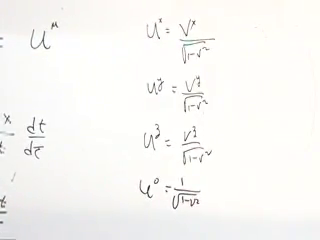
\includegraphics[width=0.82\textwidth]{lecture_05_figure_06.png}
\caption{用普通速度和洛伦兹因子表示的固有速度的四个分量。}
\lectureframe{01:34:40}
\end{figure}

恢复常规单位并使用 \(X^0=ct\)，得到标准形式
\begin{equation}
U^\mu=(\gamma_v\mathbf v,\gamma_v c)
\end{equation}
这里采用空间分量在前的排序。其不变模长为
\begin{equation}
U_\mu U^\mu=c^2.
\end{equation}
因此每个有质量粒子都具有相同不变
大小的四维速度，尽管其空间速度依赖于参考系。

\section{世界线的切矢量}

对于式~\eqref{eq:l5-four-velocity}，有一个熟悉的欧几里得模型。
沿普通三维空间中的一条曲线，
\begin{equation}
ds^2=dx^2+dy^2+dz^2.
\end{equation}
微分位移 \((dx,dy,dz)\) 沿曲线方向，但
不是单位矢量。除以弧长得到
\begin{equation}
\mathbf T=
\left(\frac{dx}{ds},\frac{dy}{ds},\frac{dz}{ds}\right),
\qquad
\mathbf T\cdot\mathbf T=1.
\end{equation}
相对论构造是同样的想法，只是用固有时代替
欧几里得弧长。矢量 \(u^\mu=dX^\mu/d\tau\) 与
世界线相切。

\begin{figure}[H]
\centering
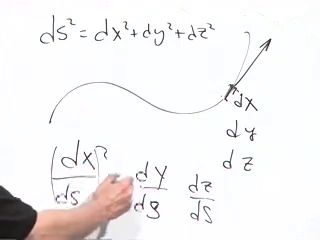
\includegraphics[width=0.82\textwidth]{lecture_05_figure_07.png}
\caption{欧几里得切矢量构造：将微分
位移除以弧长元 \(ds\)。固有时沿类时世界线扮演类似
角色。}
\lectureframe{01:39:30}
\end{figure}

\begin{classroomqa}
\audiencequestion{如果 \(c=1\)，那么固有时和固有距离相同吗？}
\lecturerresponse{令 \(c=1\) 使时间和距离具有相同单位；这
并不会消除时空几何的负号。在欧几里得类比中，
\(s\) 是沿空间曲线测量的普通距离。沿类时
世界线，\(\tau\) 是由时钟测量的流逝时间。这些构造
类似，但几何不同。}
\end{classroomqa}

再求一次导数定义固有加速度，
\begin{equation}
a^\mu=\frac{du^\mu}{d\tau}.
\end{equation}
当牛顿
第二定律被相对论化时，必须用这个量代替 \(d^2\mathbf x/dt^2\)。由于 \(u_\mu u^\mu\) 是常数，
\begin{equation}
\frac{d}{d\tau}(u_\mu u^\mu)=2u_\mu a^\mu=0,
\end{equation}
所以四维加速度与四维速度闵可夫斯基正交。\editorialnote{这种
正交性立即由不变模长得出，并作为该定义的下一项数学推论列入。}

\section{四维动量和能量}

动量是我们的最后一个例子，因为它在碰撞和衰变中守恒。
粒子具有固定的内禀质量 \(m\)，通常称为其静止质量。它
不随速度变化。相对论动量就是这个固定质量乘以
四维速度：
\begin{equation}
p^\mu=mu^\mu.
\label{eq:l5-four-momentum}
\end{equation}
在 \(c=1\) 单位下，
\begin{equation}
p^i=\gamma_v m v^i,
\qquad
p^0=\gamma_v m.
\end{equation}
在低速下 \(\gamma_v\simeq1\)，所以空间分量约化为
牛顿动量 \(m\mathbf v\)。在高速下它们比 \(m\mathbf v\) 增长得更快。

时间分量是能量。采用常规单位并使用 \(X^0=ct\)，
\begin{equation}
P^\mu=(\mathbf p,E/c)
=(\gamma_v m\mathbf v,\gamma_v mc),
\end{equation}
因此
\begin{equation}
E=\gamma_v mc^2
=mc^2\left(1-\frac{v^2}{c^2}\right)^{-1/2}.
\label{eq:l5-relativistic-energy}
\end{equation}

为了恢复普通力学，令
\(\epsilon=v^2/c^2\ll1\)。二项式展开给出
\begin{equation}
(1-\epsilon)^p=1-p\epsilon+O(\epsilon^2).
\end{equation}
取 \(p=-1/2\)，
\begin{align}
E
&=mc^2\left(1-\frac{v^2}{c^2}\right)^{-1/2}\nonumber\\
&=mc^2\left[1+\frac12\frac{v^2}{c^2}
  +O\!\left(\frac{v^4}{c^4}\right)\right]\nonumber\\
&=mc^2+\frac12mv^2+O\!\left(\frac{mv^4}{c^2}\right).
\label{eq:l5-energy-expansion}
\end{align}

\begin{figure}[H]
\centering
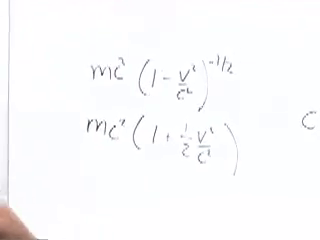
\includegraphics[width=0.82\textwidth]{lecture_05_figure_08.png}
\caption{相对论能量的低速展开，揭示出静止
能量和牛顿动能。}
\lectureframe{01:51:30}
\end{figure}

第一项 \(mc^2\) 即使在静止时也存在。在一个具有
固定粒子集合且质量不变的牛顿问题中，该项在
运动前后加上相同的常数，所以只有 \(\tfrac12mv^2\) 影响
熟悉的记账。相对论揭示出，被丢弃的常数一直都是
物理能量。

因此能量和动量并非互不相关的守恒定律。它们是
一个守恒矢量的四个分量。洛伦兹助推将它们混合：一个
观察者称为能量的东西部分地贡献给另一个观察者的动量，
反之亦然。尽管如此，对于孤立系统，总四维动量
在每个惯性参考系中于每次碰撞或衰变前后都相同。

这是相对论力学的门槛。接下来的任务是用力固有加速度来表示力，并理解相对论性波动方程，尤其是支配电磁学和光的方程。